\documentclass[14pt]{extbook}
\usepackage{multicol, enumerate, enumitem, hyperref, color, soul, setspace, parskip, fancyhdr} %General Packages
\usepackage{amssymb, amsthm, amsmath, latexsym, units, mathtools} %Math Packages
\everymath{\displaystyle} %All math in Display Style
% Packages with additional options
\usepackage[headsep=0.5cm,headheight=12pt, left=1 in,right= 1 in,top= 1 in,bottom= 1 in]{geometry}
\usepackage[usenames,dvipsnames]{xcolor}
\usepackage{dashrule}  % Package to use the command below to create lines between items
\newcommand{\litem}[1]{\item#1\hspace*{-1cm}\rule{\textwidth}{0.4pt}}
\pagestyle{fancy}
\lhead{Makeup Progress Quiz 3}
\chead{}
\rhead{Version B}
\lfoot{1648-1753}
\cfoot{}
\rfoot{Summer C 2021}
\begin{document}

\begin{enumerate}
\litem{
For the graph below, find the value(s) $a$ that makes the statement true: $ \displaystyle \lim_{x \rightarrow a} f(x)$ does not exist.
\begin{center}
    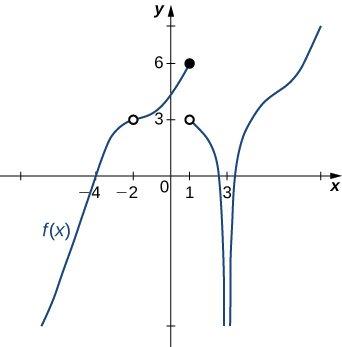
\includegraphics[width=0.5\textwidth]{../Figures/evaluateLimitGraphicallyCopyB.png}
\end{center}
\begin{enumerate}[label=\Alph*.]
\item \( -2 \)
\item \( 1 \)
\item \( 3 \)
\item \( \text{Multiple } a \text{ make the statement true}. \)
\item \( \text{No } a \text{ make the statement true}. \)

\end{enumerate} }
\litem{
Evaluate the one-sided limit of the function $f(x)$ below, if possible.\[ \lim_{x \rightarrow 8^+} \frac{-4}{(x+8)^4}+6 \]\begin{enumerate}[label=\Alph*.]
\item \( \infty \)
\item \( f(8) \)
\item \( -\infty \)
\item \( \text{The limit does not exist} \)
\item \( \text{None of the above} \)

\end{enumerate} }
\litem{
Evaluate the limit below, if possible.\[ \lim_{x \rightarrow 5} \frac{\sqrt{6x - 14} - 4}{7x - 35} \]\begin{enumerate}[label=\Alph*.]
\item \( \infty \)
\item \( 0.350 \)
\item \( 0.018 \)
\item \( 0.125 \)
\item \( \text{None of the above} \)

\end{enumerate} }
\litem{
Evaluate the limit below, if possible.\[ \lim_{x \rightarrow 6} \frac{\sqrt{6x - 20} - 4}{5x - 30} \]\begin{enumerate}[label=\Alph*.]
\item \( 0.125 \)
\item \( 0.025 \)
\item \( 0.490 \)
\item \( \infty \)
\item \( \text{None of the above} \)

\end{enumerate} }
\litem{
Based on the information below, which of the following statements is always true?
\begin{center}
    \textit{ $f(x)$ approaches $4.192$ as $x$ approaches $1$. }
\end{center}
\begin{enumerate}[label=\Alph*.]
\item \( f(1) \text{ is close to or exactly } 4 \)
\item \( f(4) \text{ is close to or exactly } 1 \)
\item \( f(4) = 1 \)
\item \( f(1) = 4 \)
\item \( \text{None of the above are always true.} \)

\end{enumerate} }
\litem{
For the graph below, find the value(s) $a$ that makes the statement true: $ \displaystyle \lim_{x \rightarrow a} f(x)$ does not exist.
\begin{center}
    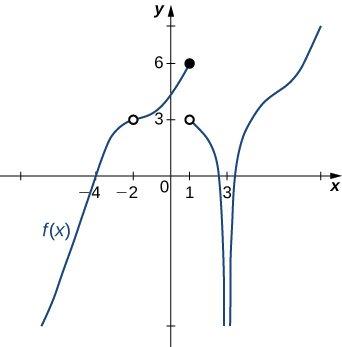
\includegraphics[width=0.5\textwidth]{../Figures/evaluateLimitGraphicallyB.png}
\end{center}
\begin{enumerate}[label=\Alph*.]
\item \( 3 \)
\item \( 1 \)
\item \( -2 \)
\item \( \text{Multiple } a \text{ make the statement true}. \)
\item \( \text{No } a \text{ make the statement true}. \)

\end{enumerate} }
\litem{
Evaluate the one-sided limit of the function $f(x)$ below, if possible.\[ \lim_{x \rightarrow -1^+} \frac{6}{(x+1)^4}+7 \]\begin{enumerate}[label=\Alph*.]
\item \( f(-1) \)
\item \( -\infty \)
\item \( \infty \)
\item \( \text{The limit does not exist} \)
\item \( \text{None of the above} \)

\end{enumerate} }
\litem{
Based on the information below, which of the following statements is always true?
\begin{center}
    \textit{ As $x$ approaches $0$, $f(x)$ approaches $15.316$. }
\end{center}
\begin{enumerate}[label=\Alph*.]
\item \( f(x) \text{ is close to or exactly } 0 \text{ when } x \text{ is close to } 15.316 \)
\item \( f(x) = 0 \text{ when } x \text{ is close to } 15.316 \)
\item \( f(x) \text{ is close to or exactly } 15.316 \text{ when } x \text{ is close to } 0 \)
\item \( f(x) = 15.316 \text{ when } x \text{ is close to } 0 \)
\item \( \text{None of the above are always true.} \)

\end{enumerate} }
\litem{
To estimate the one-sided limit of the function below as $x$ approaches 5 from the right, which of the following sets of numbers should you use?\[ \frac{\frac{5}{x} - 1}{x - 5} \]\begin{enumerate}[label=\Alph*.]
\item \( \{ 4.9000, 4.9900, 4.9990, 4.9999 \} \)
\item \( \{ 5.0000, 5.1000, 5.0100, 5.0010 \} \)
\item \( \{ 5.0000, 4.9000, 4.9900, 4.9990 \} \)
\item \( \{ 4.9000, 4.9900, 5.0100, 5.1000 \} \)
\item \( \{ 5.1000, 5.0100, 5.0010, 5.0001 \} \)

\end{enumerate} }
\litem{
To estimate the one-sided limit of the function below as $x$ approaches 6 from the left, which of the following sets of numbers should you use?\[ \frac{\frac{6}{x} - 1}{x - 6} \]\begin{enumerate}[label=\Alph*.]
\item \( \{ 5.9000, 5.9900, 6.0100, 6.1000 \} \)
\item \( \{ 6.1000, 6.0100, 6.0010, 6.0001 \} \)
\item \( \{ 6.0000, 6.1000, 6.0100, 6.0010 \} \)
\item \( \{ 6.0000, 5.9000, 5.9900, 5.9990 \} \)
\item \( \{ 5.9000, 5.9900, 5.9990, 5.9999 \} \)

\end{enumerate} }
\end{enumerate}

\end{document}